\documentclass[aspectratio=169]{beamer}
\usepackage{arydshln}
\usepackage{tikz-cd}
\usepackage[most]{tcolorbox}

\usepackage[backend=bibtex, style=authoryear, doi=false,isbn=false,url=false]{biblatex}
\bibliography{biblio_VKpres}

\usepackage{bm}
\usepackage{color}
\definecolor{theme}{RGB}{0,73,114}

\usepackage{graphicx}
\usepackage{diffcoeff}
\usepackage[most]{tcolorbox}
\usepackage{mathtools}


\setbeamertemplate{caption}{\raggedright\insertcaption\par}


\usepackage[beamer]{hf-tikz}
\usetikzlibrary{calc}

\addtobeamertemplate{footnote}{}{\vspace{2ex}}

\usepackage{xcolor}


% Syntax: \colorboxed[<color model>]{<color specification>}{<math formula>}
\newcommand*{\colorboxed}{}
\def\colorboxed#1#{%
	\colorboxedAux{#1}%
}
\newcommand*{\colorboxedAux}[3]{%
	% #1: optional argument for color model
	% #2: color specification
	% #3: formula
	\begingroup
	\colorlet{cb@saved}{.}%
	\color#1{#2}%
	\boxed{%
		\color{cb@saved}%
		#3%
	}%
	\endgroup
}

% Math macros
\DeclareMathOperator*{\grad}{grad}
\DeclareMathOperator*{\Grad}{Grad}
\DeclareMathOperator*{\Div}{Div}
\renewcommand{\div}{\operatorname{div}}
\DeclareMathOperator*{\Hess}{Hess}
\DeclareMathOperator*{\curl}{curl}
\DeclareMathOperator{\Tr}{Tr}
\DeclareMathOperator{\Dom}{Dom}
\DeclareMathOperator*{\esssup}{ess\,sup}

\newcommand{\bbR}{\mathbb{R}}
\newcommand{\bbF}{\mathbb{F}}
\newcommand{\bbA}{\mathbb{A}}
\newcommand{\bbB}{\mathbb{B}}
\newcommand{\bbS}{\mathbb{S}}

\newcommand*{\norm}[1]{\ensuremath{\left\|#1\right\|}}
\newcommand{\where}{\qquad \text{where} \qquad}


\newcommand{\inpr}[3][]{\ensuremath{( #2, \, #3 )_{#1}}}
\newcommand{\dualpr}[3][]{\ensuremath{\langle #2 \, \vert #3 \rangle_{#1}}}


\newcommand{\pder}[2]{\ensuremath{\partial_{#2} #1}}
\newcommand{\dder}[2]{\ensuremath{\delta_{#2} #1}}
\newcommand{\secref}[1]{\S\ref{#1}}
\newcommand{\energy}[1]{\frac{1}{2} \int_{\Omega} \left\{ #1 \right\} \d\Omega}
\newcommand{\crmat}[1]{\ensuremath{\left[#1\right]_\times}}
\newcommand{\fenics}{\textsc{FEniCS}\xspace}
\newcommand{\firedrake}{\textsc{Firedrake}\xspace}

\DeclareMathOperator*{\argmax}{arg\,max}
\DeclareMathOperator*{\argmin}{arg\,min}

\newtheorem{proposition}{Proposition}
\newtheorem{remark}{Remark}
\newtheorem{hypothesis}{Hypothesis}
\newtheorem{assumption}{Assumption}
\newtheorem{conjecture}{Conjecture}


\def\onedot{$\mathsurround0pt\ldotp$}
\def\cddot{% two dots stacked vertically
	\mathbin{\vcenter{\baselineskip.67ex
			\hbox{\onedot}\hbox{\onedot}}%
}}

\renewcommand\bibfont{\scriptsize}

\setbeamertemplate{navigation symbols}{}

\addtobeamertemplate{navigation symbols}{}{%
	\usebeamerfont{footline}%
	\usebeamercolor[fg]{footline}%
	\hspace{1em}%
	\insertframenumber/\inserttotalframenumber
}

\makeatletter
\g@addto@macro\normalsize{%
	\setlength\abovedisplayskip{5pt}
	\setlength\belowdisplayskip{5pt}
	\setlength\abovedisplayshortskip{5pt}
	\setlength\belowdisplayshortskip{5pt}
}
\makeatother


\makeatletter \renewcommand\d[1]{\ensuremath{%
		\;\mathrm{d}#1\@ifnextchar\d{\!}{}}}
\makeatother

\setbeamertemplate{blocks}[rounded][shadow]

\setbeamercolor{block body alerted}{bg=alerted text.fg!10}
\setbeamercolor{block title alerted}{bg=alerted text.fg!20}
\setbeamercolor{block body}{bg=structure!10}
\setbeamercolor{block title}{bg=structure!20}
\setbeamercolor{block body example}{bg=green!10}
\setbeamercolor{block title example}{bg=green!20}

\graphicspath{{./imagesVK/}}

\newif\iftocsub
\tocsubtrue
\AtBeginSection[] {
	\begin{frame}[noframenumbering]{Outline}
		\tableofcontents[sectionstyle=show/shaded, subsectionstyle=show/show/hide]
	\end{frame}
	\tocsubfalse
}
\AtBeginSubsection[] {
	\iftocsub
	\begin{frame}[noframenumbering]{Outline}
		\tableofcontents[currentsubsection, sectionstyle=show/shaded, subsectionstyle=show/shaded/hide]
	\end{frame}
	\fi
	\tocsubtrue
}

\newcommand{\beginbackup}{
	\newcounter{framenumbervorappendix}
	\setcounter{framenumbervorappendix}{\value{framenumber}}
}
\newcommand{\backupend}{
	\addtocounter{framenumbervorappendix}{-\value{framenumber}}
	\addtocounter{framenumber}{\value{framenumbervorappendix}} 
}


\begin{document}
	
	
	\begin{frame}[plain]
		
		%%%%%%%% Title slide details %%%%%%%%%%%%%%


% Background Image
\newcommand{\myBackground}
{
    
\includegraphics[height=1.02\paperheight,page=9]{beamerthemeutresources}
}

% Title
\newcommand{\myTitle}
{
A port-Hamiltonian formulation for the full von-Kármán plate model
}

% Subtitle
\newcommand{\mySubTitle}
{
}

% Author
\newcommand{\myAuthor}   
{
    Andrea Brugnoli
}

% Affiliation
\newcommand{\myAffiliate}
{
  
}

% Presentation Date
\newcommand{\myDate}   
{
    18 July 2022
}

% Logo
\newcommand{\myLogo}   
{
    
\includegraphics[width=3cm]{Logo.png}
}
%%%%%%%%%%%%%%%%%%%%%%%%%%%%%%%%%%%%


%%%%%%%%%% Title slide code %%%%%%%%%%%
\begin{tikzpicture}[remember picture,overlay]

% Background color

\fill[white] (current page.south west) rectangle (current page.north east);
% Background image
\node[above right,inner sep=0pt] at (current page.south west)
    {
        \myBackground
    };
    
% Title & Subtitle
\node
[
    above=0.5cm,
    align=center,
    draw=black!50,
    % rounded corners,
    double,
    double distance=0.1cm,
    double=blue!10,
    fill=theme!10,
    inner xsep=15pt,
    inner ysep=10pt, 
    minimum width=0.8\textwidth,
    text width=0.8\textwidth
] (title) at (current page.center)
{
    \LARGE \myTitle  \\[5pt]
    \small \mySubTitle
};

% Author 
\node[ below=0.5cm] (author) at (title.south){\myAuthor};

% Author 
\node[ below=0.25cm ](affiliate) at (author.south){\small \myAffiliate};

% Date
\node[below=0.25] (date) at (affiliate.south){\large \myDate};

% Logo
\node
[
    below =0.25cm
] at (date.south)
{
    \myLogo
};

\end{tikzpicture}
		
	\end{frame}

	
	\begin{frame}{Outline}
		
		\tableofcontents
		
	\end{frame}

\section{Why port-Hamiltonian systems?}


\begin{frame}{A unified language for multiphysics in engineering}
	The port-Hamiltonian (pH) paradigm provides a language to understand multiphysics:

	\vspace{.3cm}
	
	\begin{columns}
		\begin{column}{.65\textwidth}
			\begin{itemize}
				\item \textbf{Physics} is at the core: port-Hamiltonian systems are \textbf{passive} with respect to the \textbf{energy storage function}.
				\item The \textbf{topological} and \textbf{metrical} structure of the equation is clearly separated (mimetic discretization).
				\item PH systems are \textbf{closed under interconnection}. 
			\end{itemize}
		\end{column}
		\begin{column}{.35\textwidth}
			\centering
			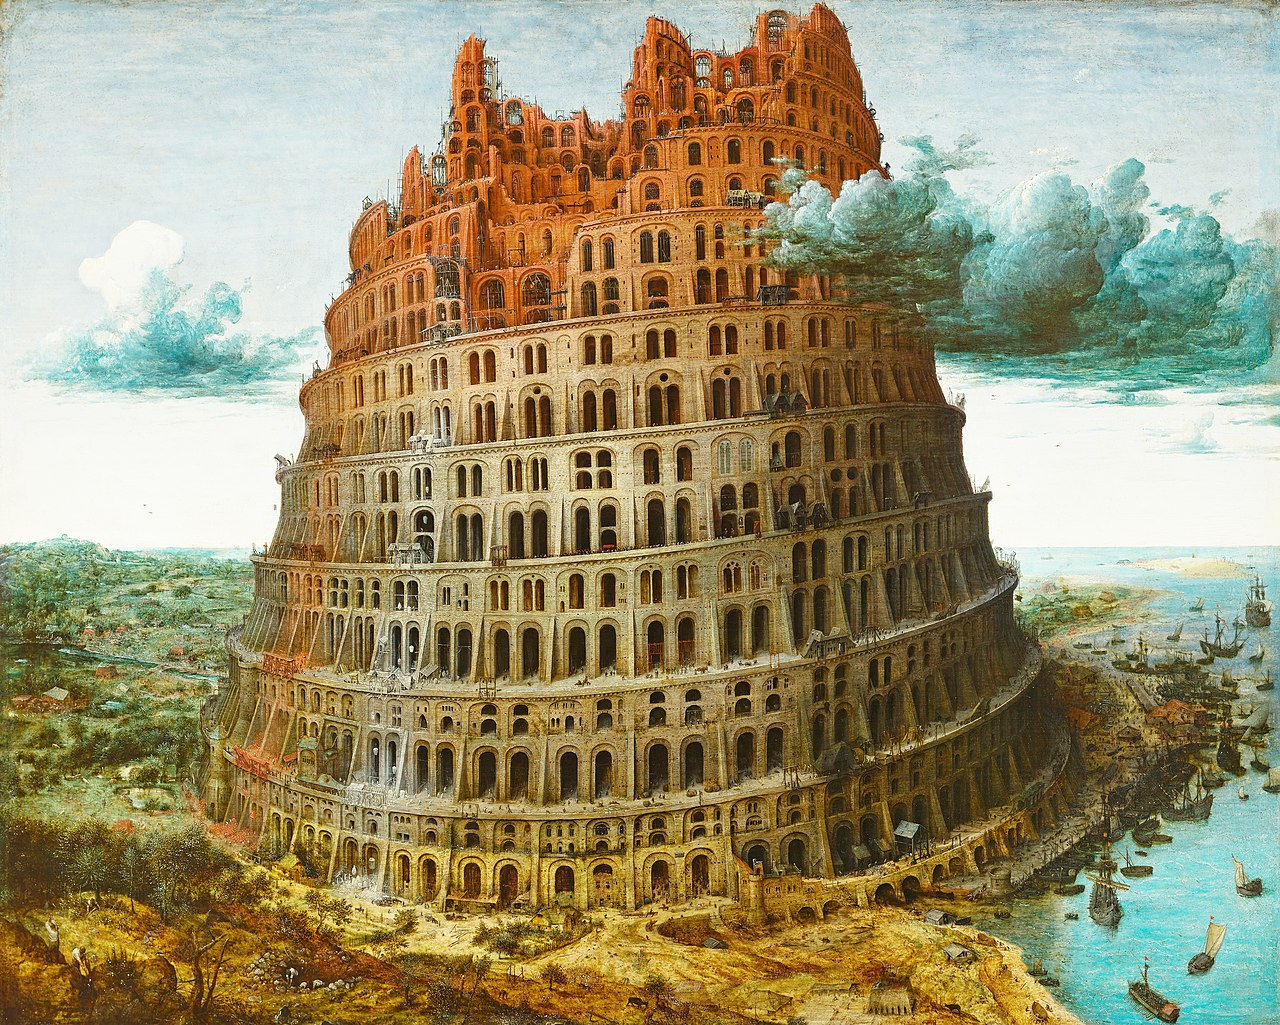
\includegraphics[width=.9\columnwidth]{babel_tower.jpeg}
		\end{column}
	\end{columns}

	
\end{frame}


\begin{frame}{Finite dimensional pH systems}
\only<1>{
	\begin{alertblock}{A theory still under developement}
		There is \textbf{not a unique definition} of pH systems, even in finite dimension.
	\end{alertblock}
	
	\begin{definition}[Finite dimensional pH system]
		
		The following time-invariant dynamical system is a pH system
		\begin{equation*}
			\begin{aligned}
				\mathbf{M}\dot{\mathbf{x}} &= \mathbf{J}(\mathbf{x})\mathbf{x} + \mathbf{B}\mathbf{u}, \\
				\mathbf{y} &= \mathbf{B}^\top\mathbf{x}.
			\end{aligned}
		\end{equation*}
		$\mathbf{x}(t) \in \mathcal{X} \subseteq \bbR^n$ is the state, $\mathbf{u}(t), \mathbf{y}(t) \in \bbR^m$ the input and output and
		\begin{itemize}
			\item $\mathbf{J}(\mathbf{x})=-\mathbf{J}(\mathbf{x})^\top \in \bbR^{n \times n}, \; \mathbf{B} \in \bbR^{n \times m}$ the interconnection and control operator.
			\item $H(\mathbf{x}) = \frac{1}{2} \mathbf{x}^\top \mathbf{M} \mathbf{x} : \mathbb{R}^n \rightarrow \mathbb{R}$ with $\mathbf{M} > 0$, the Hamiltonian.
		\end{itemize}
	\end{definition}

}
\only<2>{
\centering
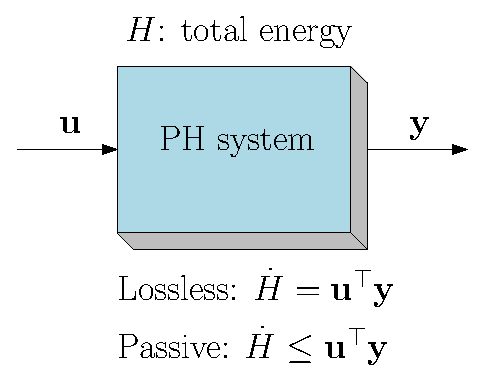
\includegraphics[width=.6\textwidth]{sketch_PH.eps}
}
	
\end{frame}


\begin{frame}{Interconnection of pH systems}

	\only<1>{
		\begin{figure}
			\centering
			\includegraphics[width=.95\textwidth]{sketch_PH_gyrator.eps}
		\end{figure}
	}
	\only<2>{
		\begin{figure}
			\centering
			\includegraphics[width=.95\textwidth]{sketch_PH_transformer.eps}
		\end{figure}
	}
	
\end{frame}

\section{Von-K\'arm\'an theory of thin beams in pH form}

\begin{frame}{Linear vs Von-K\'arm\'an plate theory}

	\begin{columns}
	\begin{column}{.5\textwidth}
			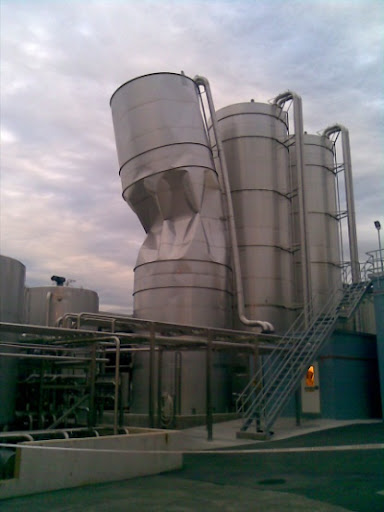
\includegraphics[width=.8\columnwidth]{buckling.jpg}
	\end{column}
	\begin{column}{.5\textwidth}

		Geometrical non-linearities allow describing bifurcations (i.e. buckling).
	\end{column}
	\end{columns}
	
\end{frame}

\begin{frame}{The von-K\'arm\'an assumption}
Second-order approximation of geometrically exact beam theory \textbf{capturing the axial bending coupling.}	

\begin{columns}
	\begin{column}{.5\textwidth}
	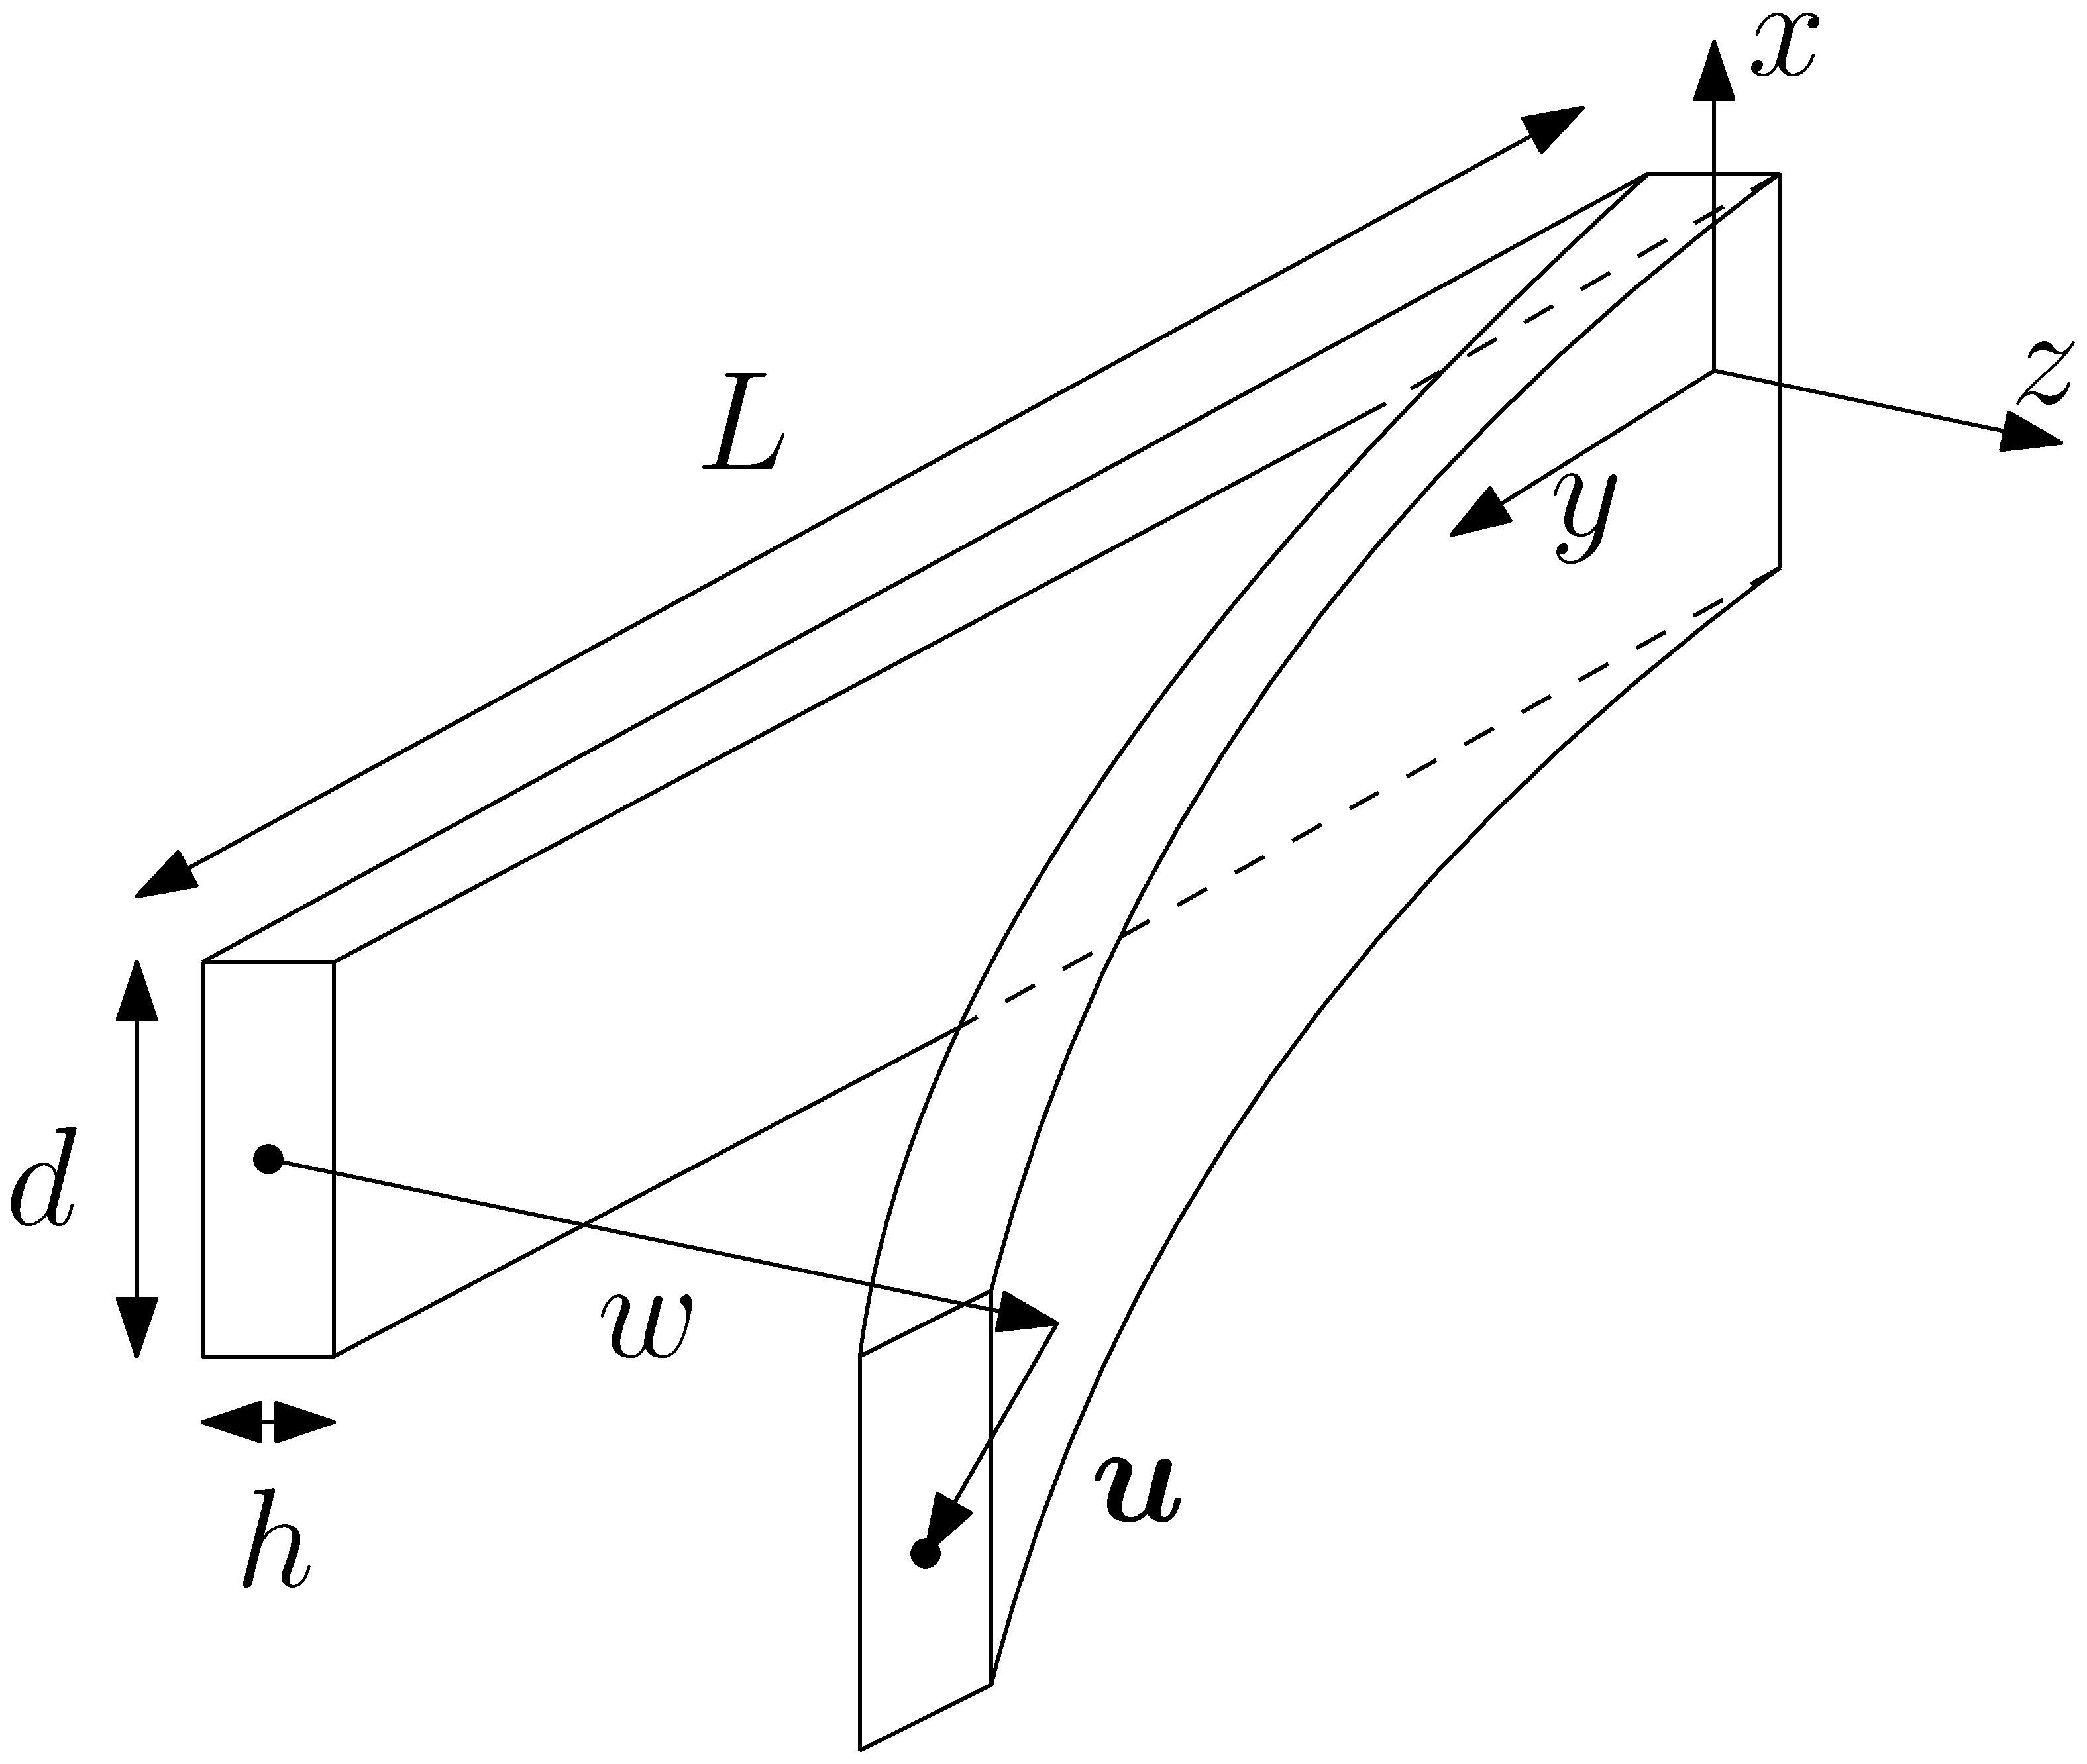
\includegraphics[width=.9\textwidth]{beam_deflected.eps}
	\end{column}
	\begin{column}{.5\textwidth}
	
	\begin{block}{Basic geometric assumption}
		\begin{itemize}
		\item Out of plane deflection comparable to the thickness: $w/h = \mathcal{O}(1)$.
		\item The squares of the in-plane stretching terms are negligible compared to the square of the rotations.
		\end{itemize}
		
	\end{block}
	
	\end{column}
\end{columns}

\end{frame}


\begin{frame}{Linear isotropic plates}
	
	The axial and bending behavior are uncoupled if $w/h \ll 1$:
	
	\begin{block}{Axial displacement (planar elastodynamics)}
		\begin{equation*}
			\rho h \partial_{tt} \bm{u} = \Div \bm{N}, \qquad \bm{N}=D_m\bm{\Phi}(\bm{\varepsilon}_m), \qquad \bm{\varepsilon}_m = \frac{1}{2} (\nabla \bm{u} + \nabla^\top \bm{u}) = \Grad \bm{u}.
		\end{equation*}
	\end{block}
	
	\begin{block}{Vertical displacement (Kirchhoff plate)}
		\begin{equation*}
			\rho h \partial_{tt} w = -\div\Div \bm{M}, \qquad \bm{M} = D_b \bm{\Phi}(\bm{\kappa}), \qquad \bm{\kappa}= \Hess w = \Grad \grad w. 
		\end{equation*}
	\end{block}
	The linear mapping $\bm\Phi (\bm{A}) = \nu \Tr(\bm{A})\bm{1} + (1 - \nu) \bm{A}$ is positive and preserves symmetry.
	
\end{frame}


\begin{frame}{Von-K\'arm\'an plates}
Decomposition strain field 
\begin{equation*}
	\bm{\varepsilon} = \tikzmarkin<1>[below right offset={0.05,-0.4},above left offset={-0.05,0.7}]{lm}\Grad \bm{u}\tikzmarkend{lm} +  \tikzmarkin<1>[below right offset={0,-0.4},above left offset={-0.05,0.7}]{nlm}1/2 \grad w \otimes \grad w\tikzmarkend{nlm} - z \; \tikzmarkin<1>[below right offset={0.05,-0.4},above left offset={-0.05,0.7}]{lb}\Hess w\tikzmarkend{lb} = \bm{\varepsilon}_m -z \bm{\kappa}.
\end{equation*}

\begin{tikzpicture}[remember picture,overlay]
	% adjust the shift from "col" to move the position of the annotation
	\coordinate (lm-a) at ($(lm)+(-1.5,-1.5)$);
	\coordinate (lm-b) at ($(lm)+(0.4,-1.1)$);
	\node[align=left] (lmstring) at (lm-a) {\small{Linear axial def.}};
	\draw[->, red](lmstring) -| node {} (lm-b);
	
	\coordinate (nlm-a) at ($(nlm)+(-2.2,-2)$);
	\coordinate (nlm-b) at ($(nlm)+(0.8,-1.1)$);
	\node[align=left] (nlmstring) at (nlm-a) {\small{Non-linear axial def.}};
	\draw[->, red](nlmstring) -| node {} (nlm-b);
	
	\coordinate (lb-a) at ($(lb)+(+2,-2)$);
	\coordinate (lb-b) at ($(lb)+(0.3,-1.1)$);
	\node[align=right] (lbstring) at (lb-a) {\small{Linear bending def.}};
	\draw[->, red](lbstring) -| node {} (lb-b);
\end{tikzpicture}
\vspace{1cm}\\

\begin{block}{Von-K\'arm\'an plate Dynamics}
	\begin{equation*}
		\begin{aligned}
			\rho A \partial_{tt}{u} &= \Div \; \tikzmarkin<1>{cp1}\bm{N}\tikzmarkend{cp1}, \\
			\rho A \partial_{tt}{w} &= -\div\Div \bm{M} + \div(\tikzmarkin<1>{cp2}\bm{N}\tikzmarkend{cp2} \grad w),
		\end{aligned} 
	\end{equation*}
Total energy $H= \frac{1}{2} \int_{\Omega} \{ D_m \bm{\Phi}(\bm{\varepsilon}_m) \cddot \bm{N} + D_b \bm{\Phi}(\kappa)\cddot \bm{M}\} \d\Omega$ 
\end{block}

\end{frame}


\begin{frame}{Port-Hamiltonian Von-K\'arm\'an plates}
	
\begin{block}{Energy and coenergy variables}
	\begin{equation*}
		\begin{aligned}
			\bm{\alpha}_u &= \rho h \partial_t \bm{u}, \\
			\alpha_w &= \rho h \partial_t{w},\\
		\end{aligned} \qquad
		\begin{aligned}
			\bm{A}_\varepsilon &= \bm{\varepsilon}_m, \\
			\bm{A}_\kappa &= \bm{\kappa}.
		\end{aligned}
	\end{equation*}
	Linear constitutive equations $\bm{e} := \delta_\alpha H = \mathcal{Q} \bm{\alpha}$ with
	\begin{equation*}
		\mathcal{Q} = \mathrm{Diag}\left[(\rho h)^{-1}, \; D_m \bm{\Phi}, \; (\rho h)^{-1}, \; D_b \bm{\Phi}\right]^{-1}.
	\end{equation*}
\end{block}

\end{frame}

\begin{frame}{The port-Hamiltonian realization}
	To close the system, variable $w$ has to be accessible. 
	\begin{equation*}
	%\diffp{}{t}
	\frac{\partial}{\partial t}
	\begin{pmatrix}
		\bm{\alpha}_u \\
		\bm{A}_\varepsilon \\
		w \\
		\alpha_w \\
		\bm{A}_\kappa
	\end{pmatrix} = 
	\underbrace{\begin{bmatrix}
			\bm{0} & \Div & \bm{0} & \bm{0} & \bm{0}\\
			\Grad & \bm{0} & \bm{0} & -\mathcal{C}(w)^* & \bm{0} \\
			0 & 0 & 0 & 1 & 0 \\
			0 & \mathcal{C}(w) & -1 & 0 & -\div\Div \\
			\bm{0} & \bm{0} & \bm{0} & \Grad\grad & \bm{0} \\ 
	\end{bmatrix}}_{\mathcal{J}}
	\begin{pmatrix}
		\delta_{\bm\alpha_u} H \\
		\delta_{\bm{A}_\varepsilon} H \\
		\delta_{w} H \\
		\delta_{\alpha_w} H \\
		\delta_{\bm{A}_\kappa} H
	\end{pmatrix},
\end{equation*}
where 
\begin{equation*}
	\begin{aligned}
		\mathcal{C}(w)(\bm{T}) &= \div(\bm{T} \grad w), \\
		\mathcal{C}(w)^*(\cdot) &= -\frac{1}{2} \left[\grad (\cdot) \otimes \grad(w) + \grad(w) \otimes \grad(\cdot) \right].
	\end{aligned}
\end{equation*}

\end{frame}


\begin{frame}{Energy rate and boundary conditions}
	
	\begin{proposition}{The energy rate reads}
	\begin{equation*}
		\dot{H} = \dualpr[\partial\Omega]{\gamma_0\bm{e}_u}{\gamma_\perp \bm{E}_\varepsilon} + \dualpr[\partial\Omega]{\gamma_0\bm{e}_w}{\gamma_{\perp\perp, 1} \bm{E}_\kappa + \gamma_0(\bm{E}_\varepsilon \bm{n} \cdot \grad w)} + \dualpr[\partial\Omega]{\gamma_1\bm{e}_w}{\gamma_{\perp\perp} \bm{E}_\kappa},
	\end{equation*}
\begin{itemize}
	\item $\gamma_0\bm{e}_u= \bm{e}_u\vert_{\partial\Omega}$ is the Dirichlet trace;
	\item $\gamma_\perp \bm{E}_\varepsilon = \bm{E}_\varepsilon \cdot \bm{n}\vert_{\partial\Omega}$ is the normal trace;
	\item $\gamma_{\perp\perp, 1} \bm{E}_\kappa = - \bm{n} \cdot \Div \bm{E}_\kappa - \partial_{\bm{s}}(\bm{n}^\top \bm{E}_\kappa \bm{s})\vert_{\partial\Omega}$ is the effective shear force;
	\item $\gamma_1 \bm{e}_w = \partial_{\bm{n}} \bm{e}_w\vert_{\partial\Omega}$ is the normal derivative trace;
	\item $\gamma_{\perp\perp} \bm{E}_\kappa = \bm{n}^\top \bm{E}_\kappa \bm{n}$ is the normal to normal trace.
\end{itemize}
	\end{proposition}

\begin{table}[h]
	Boundary conditions classification
	\centering
	\begin{tabular}{c|c|c|c}
		\hline 
		BCs & Traction & \multicolumn{2}{c}{Bending} \\ 
		\hline 
		Dirichlet BCs. & $e_u\vert_0^L$ & $e_w\vert_0^L$  & $\partial_x e_w\vert_0^L$  \\
		Neumann BCs. & $e_\varepsilon\vert_0^L$ & $e_\varepsilon \partial_x w -\partial_x e_\kappa\vert_0^L$ & $e_\kappa\vert_0^L$ \\ 
		\hline 
	\end{tabular} 
\end{table}

\end{frame}


\section{Numerical discretization}

\begin{frame}{Pure coenergy formulation}
	
	\begin{block}{Coenergy formulation for linear constitutive equations}
		If the $\mathcal{Q}$ operator is inverted:
		\begin{equation*}
			\begin{pmatrix}
				\rho A \dot{e}_u \\
				C_a \dot{e}_\varepsilon \\
				\rho A \dot{e}_w \\
				C_b \dot{e}_\kappa \\
				\dot{w} \\
			\end{pmatrix} = 
			\begin{bmatrix}
				0 & \partial_x & 0 & 0 & 0\\
				\partial_x & 0 & \partial_x w \, \partial_x & 0 & 0 \\
				0 & \partial_x(\cdot \, \partial_x w) & 0 & -\partial_{xx}^2 & -1 \\
				0 & 0 & \partial_{xx}^2 & 0 & 0 \\ 
				0 & 0 & 1 & 0 & 0 \\
			\end{bmatrix}
			\begin{pmatrix}
				e_u \\
				e_\varepsilon \\
				e_w \\
				e_\kappa \\
				\delta_w H \\
			\end{pmatrix}.
		\end{equation*}
	\end{block}
In the sequel, the quantity $\delta_w H$ is removed as no displacement dependent potential (e.g. gravity) is considered
	
\end{frame}

\begin{frame}{Weak formulation}
	
	Introducing test functions and integrating by parts the first, third and fourth, we get the weak formulation.
	
	\begin{block}{Weak formulation}
		\only<1>{Find $(e_u, e_w, e_\kappa, w) \in H^1(\Omega), \, e_\varepsilon \in L^2(\Omega)$ such that 
			\begin{equation*}
				\begin{aligned}
					\inpr[\Omega]{\psi_u}{\rho A \, \dot{e}_u} &= -\inpr[\Omega]{\partial_x \psi_u}{ e_\varepsilon} +  \inpr[\partial\Omega]{\psi_u}{e_\varepsilon}. \\
					\inpr[\Omega]{\psi_\varepsilon}{C_a \, \dot{e}_\varepsilon} &= \inpr[\Omega]{\psi_\varepsilon}{\partial_x e_u} + \inpr[\Omega]{\psi_\varepsilon}{\partial_x w \, \partial_x e_w}, \\
					\inpr[\Omega]{\psi_w}{\rho A\dot{e}_w} &= -\inpr[\Omega]{\partial_x \psi_w \partial_x w}{e_\varepsilon} + \inpr[\Omega]{\partial_{x} \psi_w}{\partial_{x} e_\kappa} \\
					&\quad +\inpr[\partial\Omega]{\psi_w}{e_\varepsilon \partial_x w - \partial_x e_\kappa}, \\
					\inpr[\Omega]{\psi_\kappa}{C_b \, \dot{e}_\kappa} &= - \inpr[\Omega]{\partial_{x} \psi_\kappa}{\partial_{x} e_w} + \inpr[\partial\Omega]{\psi_\kappa}{\partial_x e_w}, \\
					\inpr[\Omega]{\psi}{\dot{w}} &= \inpr[\Omega]{\psi}{e_w}. \\
				\end{aligned}
			\end{equation*}
			holds $\forall (\psi_u, \psi_w, \psi_\kappa, \psi) \in H^1(\Omega), \, \forall \psi_\varepsilon \in L^2(\Omega)$.}
		\only<2>{
		Find $\bm{e} =(e_u,  e_\varepsilon, e_w, e_\kappa) \in H^1\times L^2\times H^1\times H^1$ such that 
		\begin{equation*}
			\begin{aligned}
				m(\bm{\psi}, \partial_t \bm{e}) &= j_w(\bm{\psi}, \bm{e}) + b(\bm{\psi})\mathbf{u},\\
				\partial_t w &= \begin{bmatrix}
					0 & 0 & 1 & 0
				\end{bmatrix}\bm{e}, \\
				\mathbf{y} &= b^\top(\bm{e}),
			\end{aligned} 
		\end{equation*}
		$\forall \bm{\psi} \in H^1\times L^2\times H^1\times H^1:= X$
		\begin{itemize}
			\item $m$ is a symmetric, coercive, bilinear form;
			\item $j_w$ is a skew-symmetric bilinear form modulated by $w$;
			\item $b: X \rightarrow \bbR^6$ vector-valued functional.
		\end{itemize}  
	}
	\end{block}
\end{frame}

\begin{frame}{Mixed finite element construction\footcite{arnold2006acta}}
	\textcolor{blue}{Crucial concept: Hilbert complex $H^1 \xrightarrow{\partial_x} L^2$.} \\
	\begin{block}{Key requirements for mixed Galerkin approximation}
		
	\begin{itemize}
		\item The subspaces $H^1_h \subset H^1, \; L^2_h \subset L^2$ form a subcomplex $H^1_h \xrightarrow{\partial_x} L^2_h$ \hspace{1cm}(i.e. $\partial_x H^1_h \subset L^2_h$).
		\item they admit bounded linear projections $\pi_h^{H^1}: H^1 \rightarrow  
		H^1_h$  and $\pi_h^{L^2}: L^2 \rightarrow  
		L^2_h$ which commute with $\partial_x$:
		\vspace*{-\baselineskip}\vspace*{3pt}
		\[\partial_x \pi_h^{H^1} = \pi_h^{L^2} \partial_x.\]
	\end{itemize}
	\end{block}

	Satisfied for $CG_k \xrightarrow{\partial_x} DG_{k-1}$ 
	\begin{equation*}
		\begin{aligned}
			\mathrm{CG}_k &= \{u \in H^1(\Omega) | \: \forall \text{edge in the mesh}, \; u|_{\text{edge}} \in P_k\}, \\
			\mathrm{DG}_{k-1} &= \{u \in L^2(\Omega) | \: \forall \text{edge in the mesh}, \; u|_{\text{edge}} \in P_{k-1}\}, \\
		\end{aligned}
	\end{equation*}
	where $P_k$ space of polynomials of degree $k$.
	\vspace{.1cm}
\end{frame}

\begin{frame}{Finite element choice and final system}
	For the proposed weak formulation, the FE spaces become
	\begin{equation*}
			e_u^h \in \mathrm{CG}_{2k-1}, \qquad
			e_{\varepsilon}^h \in \mathrm{DG}_{2k-2}, \qquad 
			(e_w^h, \; e_\kappa^h, \; w^h) \in CG_{k}, \quad k\ge 1.
	\end{equation*}
Implications:
\begin{itemize}
	\item Subcomplex property for the linear part: $\partial_x \mathrm{CG}_{2k-1} \subset \mathrm{DG}_{2k-2}$.
	\item The non linear part respects
	$$\partial_x \mathrm{CG}_k \cdot  \partial_x \mathrm{CG}_k \subset \mathrm{DG}_{2k-2}.$$
\end{itemize}

\begin{block}{Finite dimensional system (Galerkin projection)}
		\begin{equation*}
		\begin{aligned}
			\mathbf{M} \dot{\mathbf{e}} &= \mathbf{J}(\mathbf{w})\mathbf{e} + \mathbf{B}\mathbf{u}, \\
			\dot{\mathbf{w}} &= \begin{bmatrix}
				\mathbf{0} & \mathbf{0} & \mathbf{I} & \mathbf{0} \\
			\end{bmatrix} \mathbf{e}, \\
			\mathbf{y} &= \mathbf{B}^\top \mathbf{e}.
		\end{aligned}
	\end{equation*}
\end{block}

\end{frame}


\section{Numerical convergence study}

\begin{frame}{Manufactured solution}
	The following manufactured solution is considered
	\begin{equation*}
		\begin{aligned}
			u^{\text{ex}} &= x^3[1-(x/L)^3] \sin(2 \pi t), \qquad
			w^{\text{ex}} &= \sin(\pi x/L)\sin(2 \pi t), 
		\end{aligned}
	\end{equation*}
	together with the boundary conditions
	\begin{equation*}
		u\vert_0^L = 0, \quad w\vert_0^L =0, \quad m_{xx}\vert_{0}^L=0.
	\end{equation*}
A Crank-Nicholson scheme is used for time integration.
\begin{block}{Convergence measure}
	The discrete time-space norm $L^\infty_{\Delta t} (\mathcal{X}) (\mathcal{X} = H^1 \text{or } L^2)$ is used to measure convergence
	\[
	||\cdot ||_{L^\infty (\mathcal{X})} \approx || \cdot ||_{L^\infty_{\Delta t} (\mathcal{X})} = \max_{t \in t_i} ||\cdot||_{\mathcal{X}},
	\]
	where $t_i$ are the discrete simulation instants.
\end{block}

\end{frame}

\begin{frame}{Results}
	\only<1>{
		\begin{figure}[b]
			\begin{minipage}[b]{0.58\linewidth}
				\centering
				\includegraphics[width=1\textwidth]{u_dot.eps}
				\caption{$L^\infty_{\Delta t} (H^1)$ error for $e_u$.}
			\end{minipage}
			\begin{minipage}[b]{0.4\linewidth}
				\centering
				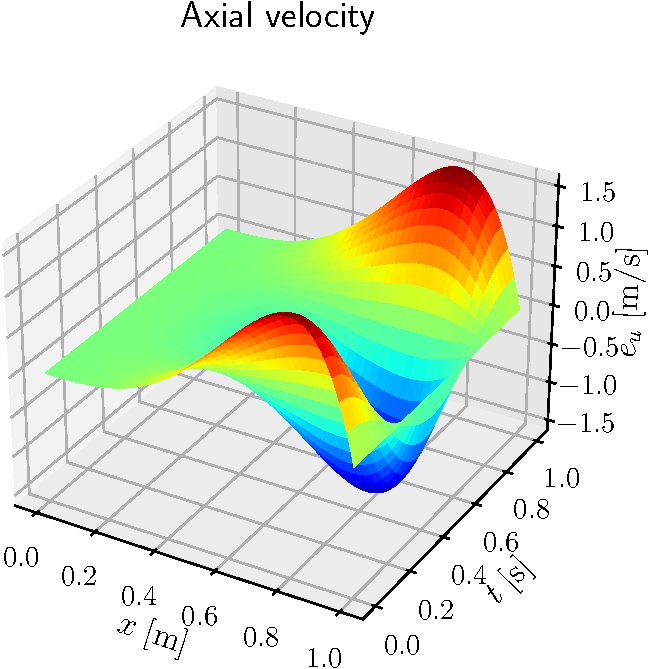
\includegraphics[width=1\textwidth]{plot_e_u_cropped.pdf}
				\caption{$e_u^h$ ($h=2^{-5}, k=2$).}
			\end{minipage}
		\end{figure}
	}
	\only<2>{
		\begin{figure}[b]
			\begin{minipage}[b]{0.58\linewidth}
				\centering
				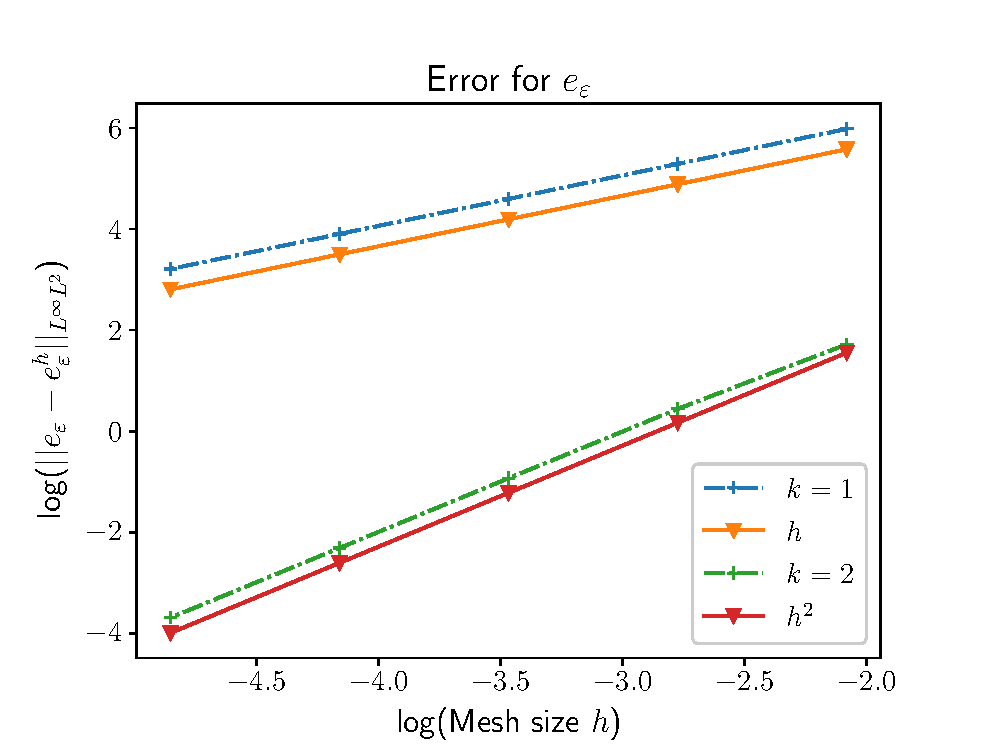
\includegraphics[width=1\textwidth]{n_xx.eps}
				\caption{$L^\infty_{\Delta t} (L^2)$ error for $e_\varepsilon$.}
			\end{minipage}
			\begin{minipage}[b]{0.4\linewidth}
				\centering
				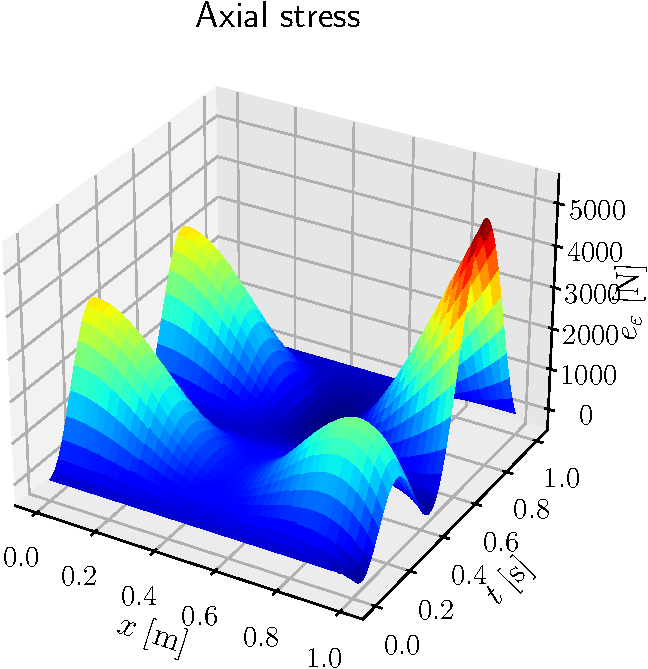
\includegraphics[width=1\textwidth]{plot_e_eps_cropped.pdf}
				\caption{$e_\varepsilon^h$ for $h=2^{-5}, k=2$.}
			\end{minipage}
		\end{figure}
	}
	\only<3>{
		\begin{figure}[b]
			\begin{minipage}[b]{0.58\linewidth}
				\centering
				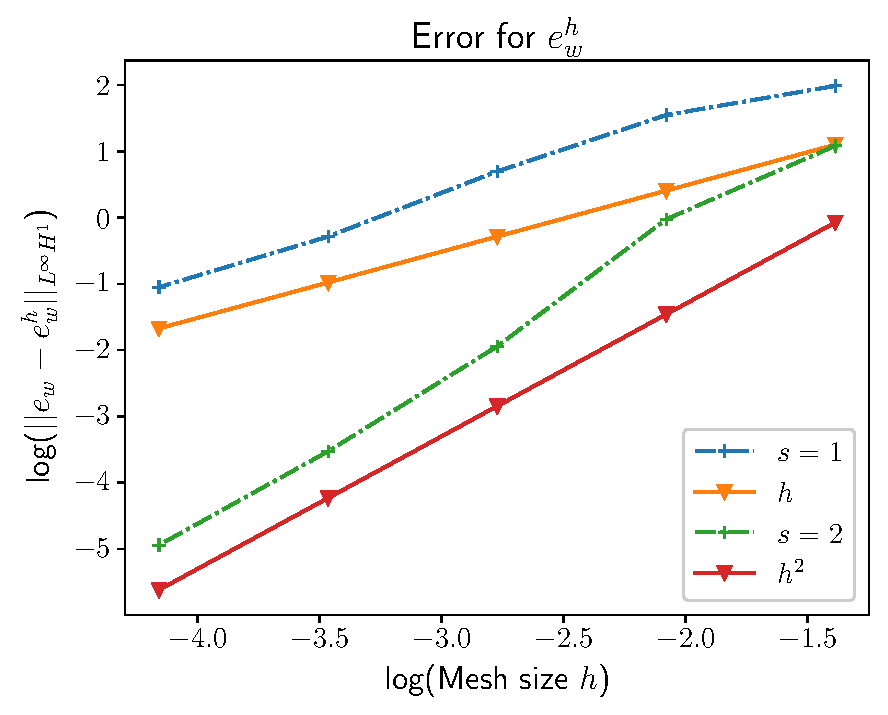
\includegraphics[width=1\textwidth]{w_dot.eps}
				\caption{$L^\infty_{\Delta t} (H^1)$ error for $e_w$.}
			\end{minipage}
			\begin{minipage}[b]{0.4\linewidth}
				\centering
				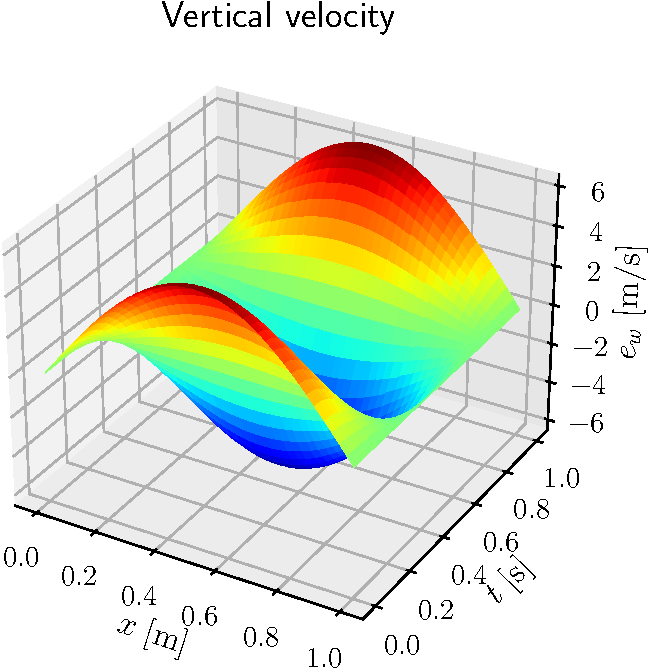
\includegraphics[width=1\textwidth]{plot_e_w_cropped.pdf}
				\caption{$e_w^h$ for $h=2^{-5}, k=2$.}
			\end{minipage}
		\end{figure}
	}
	\only<4>{
		\begin{figure}[b]
			\begin{minipage}[b]{0.58\linewidth}
				\centering
				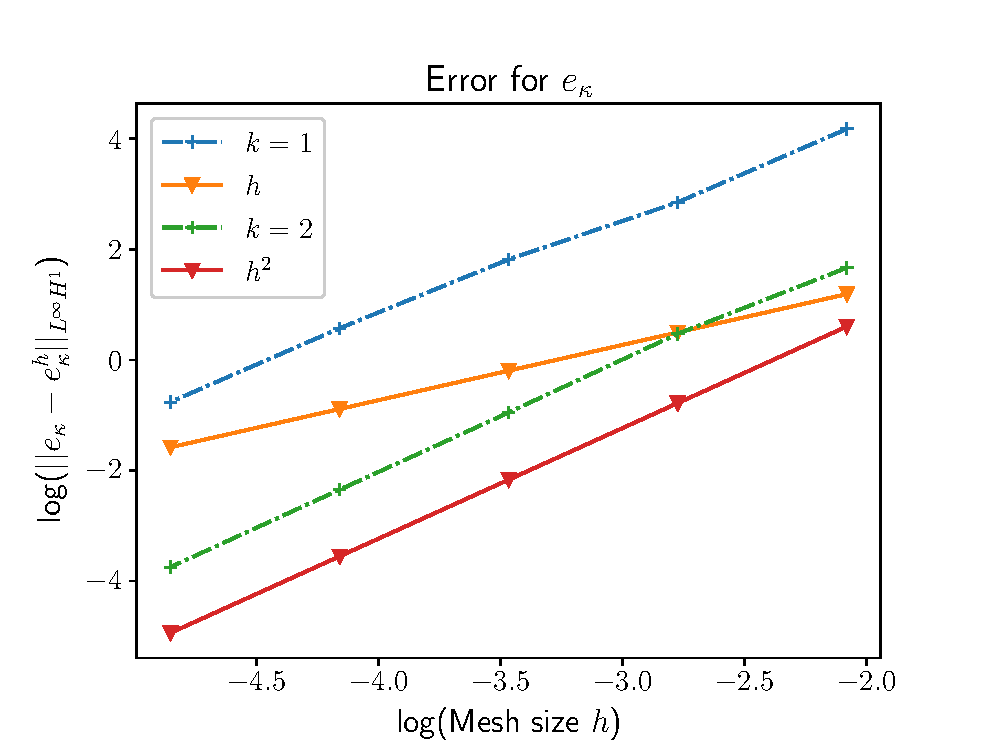
\includegraphics[width=1\textwidth]{m_xx.eps}
				\caption{$L^\infty_{\Delta t} (H^1)$ error for $e_\kappa$.}
			\end{minipage}
			\begin{minipage}[b]{0.4\linewidth}
				\centering
				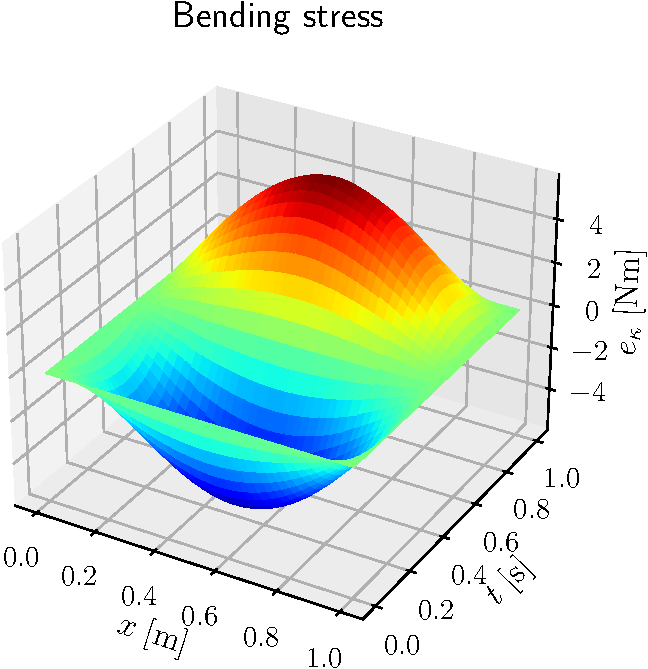
\includegraphics[width=1\textwidth]{plot_e_kap_cropped.pdf}
				\caption{$e_\kappa^h$ for $h=2^{-5}, k=2$.}
			\end{minipage}
		\end{figure}
	}
\end{frame}

\begin{frame}{Conclusion and Outlook}
\begin{itemize}
	\item First step into pH non linear mechanics. The geometrical non linearities belong to the interconnection operator.
	\item Natural extension for the 2D case (fancier FE).
	\item Can be used to study more complex phenomena. The discretization method guarantees energy conservation.
\end{itemize}
\end{frame}

\begin{frame}[allowframebreaks]{References}\label{lastslide}
	\printbibliography
\end{frame}


\begin{frame}{Port-Hamiltonian von-K\'arm\'an plates}
	\begin{equation*}
		%\diffp{}{t}
		\frac{\partial}{\partial t}
		\begin{pmatrix}
			\bm{\alpha}_u \\
			\bm{A}_\varepsilon \\
			w \\
			\alpha_w \\
			\bm{A}_\kappa
		\end{pmatrix} = 
		\underbrace{\begin{bmatrix}
				\bm{0} & \Div & \bm{0} & \bm{0} & \bm{0}\\
				\Grad & \bm{0} & \bm{0} & -\mathcal{C}(w)^* & \bm{0} \\
				0 & 0 & 0 & 1 & 0 \\
				0 & \mathcal{C}(w) & -1 & 0 & -\div\Div \\
				\bm{0} & \bm{0} & \bm{0} & \Grad\grad & \bm{0} \\ 
		\end{bmatrix}}_{\mathcal{J}}
		\begin{pmatrix}
			\delta_{\bm\alpha_u} H \\
			\delta_{\bm{A}_\varepsilon} H \\
			\delta_{w} H \\
			\delta_{\alpha_w} H \\
			\delta_{\bm{A}_\kappa} H
		\end{pmatrix},
	\end{equation*}
where 
\begin{equation*}
	\begin{aligned}
		\mathcal{C}(w)(\bm{T}) &= \div(\bm{T} \grad w), \\
		\mathcal{C}(w)^*(\cdot) &= -\frac{1}{2} \left[\grad (\cdot) \otimes \grad(w) + \grad(w) \otimes \grad(\cdot) \right].
	\end{aligned}
\end{equation*}

\end{frame}




\end{document}

